\documentclass{sig-alternate}

\begin{document}

\title{Chemoinformatics: The Computer Science of Chemistry}
\numberofauthors{3}
\author{
\alignauthor
Ben Trovato\titlenote{Dr.~Trovato insisted his name be first.}\\
       \affaddr{Institute for Clarity in Documentation}\\
       \affaddr{1932 Wallamaloo Lane}\\
       \affaddr{Wallamaloo, New Zealand}\\
       \email{trovato@corporation.com}
% 2nd. author
\alignauthor
G.K.M. Tobin\titlenote{The secretary disavows
any knowledge of this author's actions.}\\
       \affaddr{Institute for Clarity in Documentation}\\
       \affaddr{P.O. Box 1212}\\
       \affaddr{Dublin, Ohio 43017-6221}\\
       \email{webmaster@marysville-ohio.com}
% 3rd author
\alignauthor
Rajarshi Guha\\
\affaddr{NIH Center for Translational Therapeutics}\\
\affaddr{9800 Medical Center Drive}\\
\affaddr{Rockvile, MD 20850}\\
\email{guhar@mail.nih.gov}
}

\additionalauthors{Additional authors: John Smith (The Th{\o}rv{\"a}ld Group,
email: {\texttt{jsmith@affiliation.org}}) and Julius P.~Kumquat
(The Kumquat Consortium, email: {\texttt{jpkumquat@consortium.net}}).}
\date{30 July 1999}

\maketitle
\begin{abstract}
  One of the most prominent success stories in all of science over the last decade has
  been the advance of bioinformatics: interdisciplinary collaboration between
  computer scientists and molecular biologists led to the sequencing the human genome
  (among many other accomplishments), because researchers connected biological
  technologies to the theory of string algorithms. However, despite this great
  success, few computer scientists are familiar with a related (and older!)
  discipline -- chemoinformatics, the use of computers to discover new molecules with
  desired behavior, such as new pharmaceuticals or industrial solvents. Until
  recently, the data and techniques of chemoinformatics have been closely guarded
  secrets of companies whose financial success depended on being the first to produce
  the new "miracle molecule". Only within the last decade -- and largely because of
  chemists volunteering their time for an Open Science "movement" -- do researchers
  now have access to freely available software packages and databases of tens of
  millions of chemicals. As a result, chemists now confront hundreds of unsolved
  algorithmic problems that could not have been tackled a decade ago, but whose
  solutions are critical to research ranging from determining the behavior of small
  molecules in biological pathways, to finding a cure for malaria.
\end{abstract}

\category{H.4}{Information Systems Applications}{Miscellaneous}
\terms{Theory}
\keywords{cheminformatics, graphs, chemistry}

\section{Is Cheminformatics the New Bioinformatics?}

Novel technologies in the life sciences churn out information at an ever
increasing rate – public data stores such as at the European Bioinformatics
Institute (EBI) contain on the order of 10 Petabytes of biological information,
a long way from the few kilobytes of the first sequenced genome in 1977.
However, while biological information has been available publicly for decades,
the same has not been true for chemical information until very recently. Only
2004 saw a large public compound repository, PubChem, entering the public
domain, followed more recently by other databases as discussed later in this
article. In the same vein, open source software and the publication of
algorithms have only recently become a main focus of the field \cite{faulon2010}.

So why should we actually care about chemical information being made public --
and how does this relate to the field of computer science?

Both of these questions have relatively straightforward answers. We should care
about chemical information being made public since the drugs we take are the
result of intensive and costly research, and the more information is shared (a
process sometimes very hard to achieve in pharmaceutical companies) the more
easy it should be to develop novel treatments drugs. How chemical information
relates to computer science becomes clear when realizing the amount of data
available currently – 74 million different molecules with annotations are
currently stored in public databases such as PubChem with a large amount of
annotations, and the design of data structures for chemicals, as well as
subsequent data mining of this information, are areas where expertise in
computer science is dearly needed. (For a recent, detailed introduction to the
field written for computer scientists see \cite{brown2009} .) Cheminformatics comprises
different areas, which broadly speaking can be divided into three fields:
capturing data (using lab notebooks or potentially using formats such as the
Chemical Markup Language for publications); storing data (designing database
schemas, devising ontologies) and mining data (such as for bioactivity
prediction, which might involve algorithms based on graphs). However, what is a
major difference to the bioinformatics field is the type of information being
analyzed: While bioinformatics often deals with sequences, the domain of
cheminformatics is chemical structures. In case of the former, information can
very frequently be represented as one-dimensional strings, which are relatively
easy to handle computationally. On the other hand, chemical structures may
possess rings, branches as well as multiple valid representations of even the
same structure, potentially giving rise to ambiguities. Hence, chemical
structure is often thought of as being more difficult to standardize than
information from other domains. As an illustration, different representations of
the same chemical structure are shown in Figure 1. The top left hand corner
shows a structure a chemist would draw it – every ‘corner’ representing a carbon
atom (which can also be represented as a C), every O denoting oxygen, every N
nitrogen, every H hydrogen and so on. This is the standard format chemists use
when exchanging information with their peers. However, this is not directly
amenable to data mining -- different atoms might be collapsed into one node, sets
of atoms might have the same relevant properties assigned. Hence, the top right
hand corner of Figure 1 shows an annotated graph representation, taking into
account that atoms, though being of different elemental atom type, can have
similar properties -- e.g. both oxygen and nitrogen carry an 'On' label in this
graph.

\begin{figure}
\centering
\psfig{file=placeholder.ps}
\caption{The many different facets of representing chemical structures. Shown
are a chemist’s usually representation of a molecule (top left) and a
graph-based representation amenable to data mining (top right). These
representations are supplemented by a 3D representation of the same molecule
(bottom left) that is closer to reality and a representation using surface
properties (bottom right), which is often more relevant for the properties the
molecule exhibits in an experimental setup (such as when measuring its
solubility, or bioactivity).}
\end{figure}

On this graph, and employing large databases of thousands of molecules, graph
mining algorithms can be applied to discover patterns in large-scale datasets
and a large number of successful applications of this concept have been
published \cite{wegner2006,horst2009}. Still, this second representation is far
from being the end of the story. Molecules are 3D entities as represented in the
bottom left hand corner of the figure, and the precise 3D shape is relevant in
many situations (while not in others), but this is information that is lost when
only considering the graph of a molecule. To even extend this concept, in many
cases actually the surface properties of theq molecule are what appears to be
relevant in e.g. biological systems, as shown in the bottom right hand corner.
Hence, while graph mining on chemicals is certainly a promising avenue to
explore, one needs to keep in mind that not all molecular properties are encoded
in the graph (such as rotational states, or different charge states etc.) and
thus often other 'descriptors' need to be used to capture the essentials of a
chemical system \cite{bender2004}.

From the above it becomes clear that the nature of chemical problems is often a
complex mixture of combinatorial and continuous problems. If we oversimplify the
nature of chemical structures and their properties we can not describe the world
around us in sufficient details. On the other hand, if we try encoding all
details the complexity to collect, store, and mine data increases dramatically
(e.g. all possible 3D structures and their properties, all metabolites of a
structure in humans in different tissues). For the field of cheminformatics to
flourish, we need closer collaboration between chemists (or, more generally,
life scientists) and computer scientists – where the former needs to be able to
pose the problem in a way relevant for practical applications; and where the
latter is able to devise ways of capturing, storing, and analyzing chemical data
by bridging the gap between risk in generalizable encodings and complexity
(space and time). The goal is supporting a better chemical decision making by
reducing the risks by 1. storing and integrating data in maintainable ways, 2.
providing enough open standards and tools to allow software engineering concepts
to help bridging silos, and 3. mining the many chemical property spaces in a
time and space efficient way. Many aspects pertaining to those areas will be
discussed in the following sections.

\section{Bridging Cheminformatics \& Computer Science}
\label{sec:bridg-chem-}

\subsection{Databases \& Ontologies}
\label{sec:datab--ontol}


\bibliographystyle{srt,abbrv}  
\bibliography{paper}  

\end{document}